% TO DO
% Ricercare la parola TUTORIAL, per capire se nel tutorial di AkyV ci siano delle esclusioni a priori che in realtà io approfondirò nel libro
\documentclass[12pt, letterpaper]{book}

\usepackage{imakeidx}

\usepackage[obeyspaces]{url}

\usepackage[english]{babel}

\usepackage[backend=biber]{biblatex}
\usepackage{csquotes}
\addbibresource{references.bib}

\usepackage{graphicx}

\usepackage{hyperref}
\hypersetup{
    colorlinks=true,
    linkcolor=blue,
    filecolor=magenta,      
    urlcolor=cyan,
    pdftitle={Tomb Editor and Tomb Engine - An introduction by rickyturaz},
    pdfpagemode=FullScreen,
    }

\usepackage{amsthm}
\newtheorem*{remark}{Remark}

% \usepackage{luacode}
\usepackage{listings,xcolor}

\lstdefinestyle{lua}{
  language=[5.1]Lua,
  basicstyle=\ttfamily,
  keywordstyle=\color{magenta},
  stringstyle=\color{blue},
  commentstyle=\color{black!50}
}

\usepackage[os=win]{menukeys}

\title{\emph{Tomb Editor and Tomb Engine} \\ An introduction}
\author{rickyturaz}

\makeindex
\begin{document}

\maketitle
\chapter*{Preface}
% La prefazione è da scrivere alla fine. Spiega il motivo per cui hai scritto il manuale ed a chi è rivolto.
% Spiegando a chi è rivolto, inserire qui i concetti fondamentali relativi a Tomb Raider, da sapere. Ad esempio, se parlo di TR4 devi sapere di cosa si parla. Scherzaci un po' su: se sei qui a leggere questo manuale, un po' Lara ti deve piacere, no?! :)
\chapter*{Legal disclaimer}
\textbf{Tomb Engine} uses modified MIT license for non-commercial use only. For more information, see \href{https://github.com/TombEngine/TombEngine?tab=License-1-ov-file#readmeense}{license}. Tomb Engine is unaffiliated with the Crystal Dynamics group of companies or Embracer Group AB.
\par \textbf{Tomb Raider} is a trademark of the Crystal Dynamics group of companies. Tomb Engine team is not responsible for illegal use of Tomb Engine source code and built binaries alone or in combination with third-party assets or components. Tomb Engine source code is released as-is and continues to be maintained by non-paid contributors in their free time.
\tableofcontents

\part{Introduction}
\chapter{History of Tomb Raider Level Editors}
\section{Back to 2000: \emph{Tomb Raider Level Editor} \index{Tomb Raider Level Editor}\index{TRLE}}
Tomb Raider marked a sensational new approach to 3rd person gaming. Fans not only fell in love with Lara and her moves, but with the imaginative and intriguing worlds of her adventures. It all started with Lara's visit to some Egyptian ruins back in 1996, and now with the release of the Tomb Raider Level Editor has come full circle, offering a different sort of adventure in another Egyptian setting. \emph{Tomb Raider Chronicles} marks the end of the line of Tomb Raider games made with these development tools; but rather than viewing this as an end, the release of the editor makes it seem more like a beginning...
\par The \textbf{Tomb Raider Level Editor (TRLE)} includes a tutorial that will walk you through the basics needed to create your own stand alone Tomb Raider levels (but please read the legal disclaimer about commercial use of this product). Even though you will not be able to edit objects or animations (that means Lara’s outfits), you have a wonderful variety of object sets from which to choose. You can sculpt and design on many different ‘levels’ – trigger events, create awe-inspiring spaces, simple to complex…and as you experiment you will learn more about what can be done, and quite possibly discover new methods of applying the knowledge you have acquired.
\par We sincerely hope you will enjoy inventing, designing, and building with and for Lara as much as we have over the past 4 years. We thank all those who have held the enthusiasm for the Tomb Raider series, thereby contributing to its success. We wish you happy adventuring with Lara and the tools used to create her worlds.
\cite{trle_manual}
\section{Paolone's \emph{Next Generation Level Editor} \index{NGLE} \index{Next Generation Level Editor}}
The \textbf{Next Generation Level Editor}, often abbreviated \textbf{NGLE}, is a modified version of the Tomb Raider Level Editor, created by Paolone, and released in January 2007. \cite{wikiraider_NGLE}
\par Tomb Raider Next Generation \index{Tomb Raider Next Generation} (TRNG) \index{TRNG} tools, improve the TRLE tools used to build custom levels with the engine, supplied by Eidos, of Tomb Raider - The Last Revelation.
\par Many objects have beed added, some imported by other TR adventures, like boat or frog-man, other builded ex-novo like Detector or Elevator.
\par There is a new scripter program named NG\_Center. This program other to build your script.dat supplies other little tools. \cite{paolone_trng}
\section{MontyTRC89's \emph{Tomb Editor}}
\textbf{Tomb Editor (TE)} is a level editor designed for the full range of classic Tomb Raider game series (1-5), as well as for contemporary engine reimplementation projects and game engines designed for community modding and level building. \cite{TE_github}

\chapter{Basic concepts to know about Tomb Raider}
% Inserire qui i concetti fondamentali relativi a Tomb Raider, da sapere. Ad esempio, se parlo di TR4 devi sapere di cosa si parla. Scherzaci un po' su: se sei qui a leggere questo manuale, un po' Lara ti deve piacere, no?! :)
\part{Getting started}
\chapter{Installing Tomb Editor}
First of all, you need to download and install the Tomb Editor pack on your computer. wIt is available eg. \href{https://tombengine.com/}{here}.
\par The default route of Tomb Editor installed is \path{C:\Tomb Editor}. The contents of this main folder are:
\begin{itemize}
    \item Tomb Editor program.
    \item Side programs dedicated to Tomb Editor: SoundTool, TombIDE, WadTool.
    \item Most of the files which are necessary to start a basic project and level for Tomb Engine. (But texture files for room faces must be find somewhere else. But this is still not necessary now, when you start reading this tutorial.)
    \item Other important files for Tomb Editor pack.
\end{itemize}
So when you have the Tomb Editor pack installed on your computer, then you are just ready to start building levels for Tomb Engine. \cite{akyv_tutorial}

\chapter{Starting a new project}
After the installation of Tomb Editor pack, you are ready to make your very first Tomb Engine project. (Level map file extensions are well-known as “PRJ” files, but do not misunderstand: what we call “project” now is not a level, but a whole level set - i.e. your current Tomb Engine game itself, which will be released when you fully made it.)
\par But where do you need to place your projects? Well, NOT in Tomb Editor main folder - that is a place you usually never modify while editing. I suggest placing all of your projects nicely collected in a so-called general project folder. This could be called eg. \path{"My_Tomb_Raider_projects"}, created manually. (I created it in Documents folder.)
\par Each project you make will be placed in its own main folder. Does it mean now you should also create manually a project main folder in the general folder? No, there is a TombIDE wizard which will do the whole project-creating procedure for you.
\par Projects are handled in \textbf{TombIDE (Tomb Integrated Development Environment or TIDE)} program, that is why the whole project-creating procedure is also being done there.
So start \path{TombIDE.exe}, and the panel of TIDE Start page opens up.
Click on “Create a new project” button now.
The first page of a new panel opens up (General Information, \ref{fig:tide1}):
\begin{figure}
    \centering
     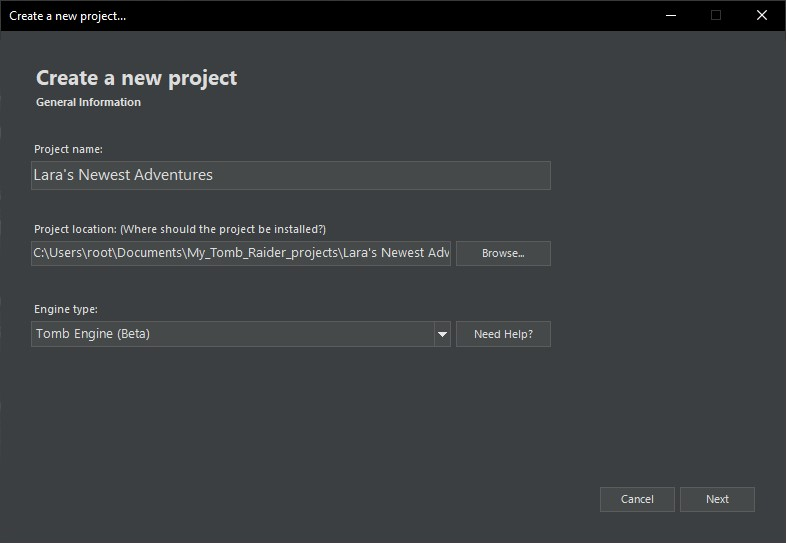
\includegraphics[width=0.75\textwidth]{screenshots/1.jpg}
     \caption{General Information}
     \label{fig:tide1}
\end{figure}

\begin{itemize}
    \item Let's suppose the project you start now has the name of “Lara's Newest Adventures”. So type it now here.
    \item Click on “Browse” button, find and select the general project folder.
    \item After that, the little window in the middle of this first page shows that a subfolder in the general project folder will be created as the main folder of this project, having the project name.
    \item The engine type you choose now is naturally Tomb Engine.
\end{itemize}


\par Now click on “Next” button to continue the procedure on the next page of the panel (Extra Options, \ref{fig:tide2}).

\begin{figure}
    \centering
     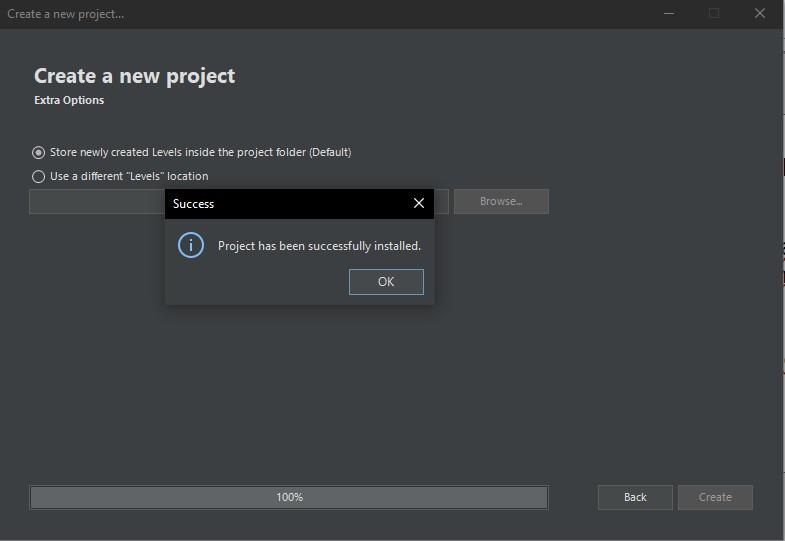
\includegraphics[width=0.75\textwidth]{screenshots/2.jpg}
     \caption{Extra Options}
     \label{fig:tide2}
\end{figure}

\par I suggest changing nothing here. Which means level map files will be handled in a folder called "Levels", which is a subfolder in the main folder of the project. (I mean, this is the default place for level map files, and you, the beginner probably should keep it like this.)
\par Now click on "Create" button here, then look at the increasing bar at the bottom of the panel.
When the bar is at 100 \%, then you get a message that the project has been successfully created (\ref{fig:tide3}).

\begin{figure}
    \centering
     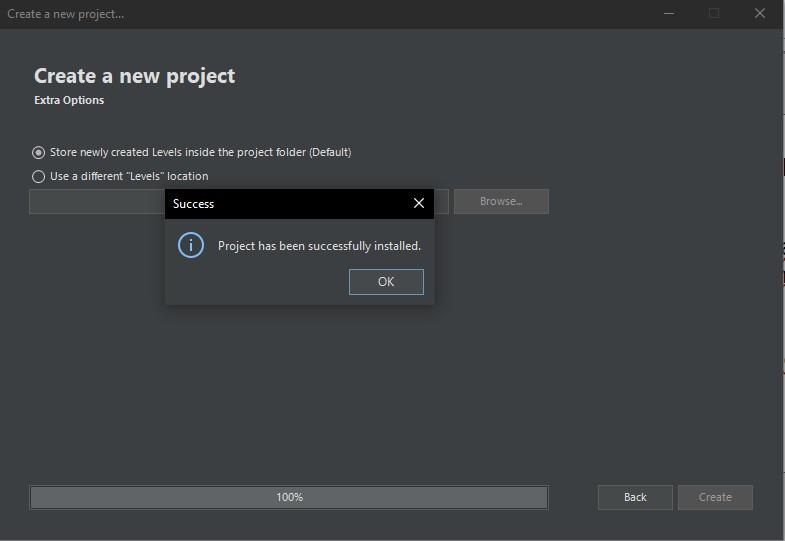
\includegraphics[width=0.75\textwidth]{screenshots/3.jpg}
     \caption{Project has been successfully installed}
     \label{fig:tide3}
\end{figure}

\par And this project main folder has been also created on the selected route, with the basic contents a TEN project should have. (Including Levels folder - still being empty - in that default position., \ref{fig:tide4})

\begin{figure}
    \centering
     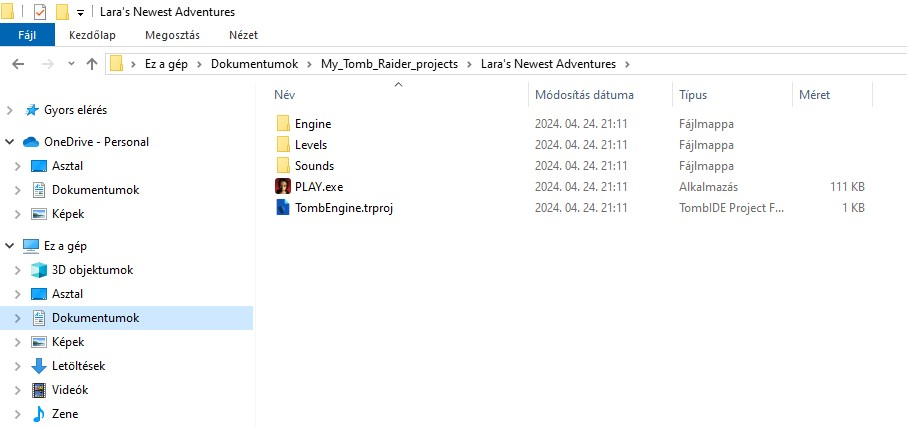
\includegraphics[width=0.75\textwidth]{screenshots/4.jpg}
     \caption{Project directories have been created (Since TEN 1.7., the project main folder has an Assets subfolder as well.)}
     \label{fig:tide4}
\end{figure}

Double-click on that row (or click on "Open selected button" below), so the project opens in TIDE, you will be able to work on it. Each project opened in TIDE has more pages, now you can see its Level Manager page. (See the panel header which names the current project.)
\par Now click on the red arrow in the upper left corner of the page, to go back to TIDE Start page, closing this project now in TIDE. (Since TEN 1.7., you can see the blue TIDE icon in that corner, instead of the red arrow. If you click on that icon, then a menu opens. One of the menu options is an arrow, with "Back to Start Window..." name. Click on it to go back to TIDE Start page.) \cite{akyv_tutorial}

\part{Rooms: floors and ceilings}

\chapter{Introduction}

\section{Blocks, sectors and clicks}

\textbf{Blocks, squares, sectors and clicks}: get used to these terms because you'll hear them frequently. The Tomb Editor is designed to work with a basic \emph{building block}, proportioned to Lara and her movements.
\par Levels are built by connecting a series of rooms comprised of walls and building blocks. The floor and ceiling of these rooms are sectioned into squares or sectors. The building blocks are created when you raise a square up from the floor or lower one down from the ceiling. Four mouse clicks up or down equals the width of these squares sections and creates a perfect cube \emph{Remember all those "blocks" Lara pushed and pulled around?!}
\par The building blocks are not limited to cubes and columns with flat tops. Corners of the surfaces can be pulled up or down to create angled slopes and \emph{organic} surfaces - great for creating rocky caves or sand dunes. \cite{trle_manual}

\section{Basic definitions}

Let's start with the default room: in the previous part, we've learnt that when we create a new level, TombIDE creates for us a level containing one room having size 18x18x3. Ok but.. 18x18x3 what?

It's time to introduce some formal definitions, forming a common dictionary.

\begin{remark}
    Property of a room is its \textbf{area}, measured in \emph{sectors} or \emph{squares}. This corresponds to the area of room's floor and room's ceiling, excluding walls.
\end{remark}

For our default room, its area is 18 squares. We can check it by alternatively counting squares in the Editor Windows, looking at the Sector Options or switching to the 2D mode in Tomb Editor.

Please note in the 3D view:
\begin{itemize}
    \item in the main editor window, floor and ceiling are represented in light blue color, while walls are represented in green;
    \item in the Sector Options panel, floor and ceiling are represented in light blue color, while walls are represented in grey.
\end{itemize}

\begin{remark}
    Given a room, the area of its floor is equal to the area of its ceiling.
\end{remark}

\begin{remark}
    Number of floor sectors is equal to number of ceiling sectors.
\end{remark}

Now, recall in mind a way to define position of objects in the three-dimensional space we live our life: we can rely on the cartesian coordinate system, where we use the three axes \( x, y, z\).
Up to now, we cared about \(x\) and \(y\). Let's introduce the way we can set \(z\) coordinate (height) and so, clicks:

\begin{remark}
    A \textbf{click} or full step is a linear transformation can be applied to a floor or a ceiling sector to increase or decrease its height.
\end{remark}

By using clicks, we can make a block.

\begin{remark}
    A \textbf{block} is the solid shape we can obtain by applying clicks to floor (raising) or ceiling (lowering).
\end{remark}

Finally, we reach the definition of the \emph{Tomb Raider cube}:
\begin{remark}
    A \textbf{Tomb Raider cube} is a cube-shaped block, where every edge is 4 clicks long.
\end{remark}

The definition of the Tomb Raider cube is useful because it's a simple way to remember Lara's sizes compared to her world and the real world.
Let's compare Lara's sizes and her movements with the cube, to better understand (\ref{fig:TIDELaraAndCube}).

\begin{remark}
    Lara's height is \emph{3 clicks}.
\end{remark}

\begin{remark}
    Assuming Lara's real height is 1.80m according to the original story \cite{wikiraider_LaraCroft}, a \emph{click} is 60cm and a \emph{Tomb Raider cube} is 2.40m high.
\end{remark}

\begin{figure}
    \centering
     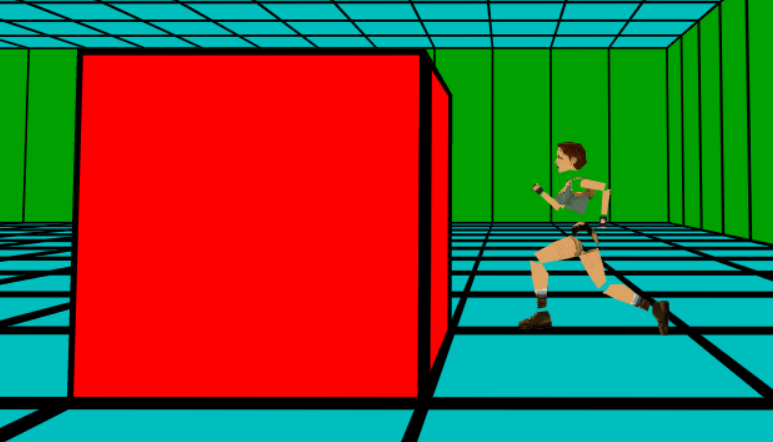
\includegraphics[width=1\textwidth]{screenshots/1010.png}
     \caption{Lara compared to the Tomb Raider cube.}
     \label{fig:TIDELaraAndCube} 
\end{figure}

In the next chapter we'll check together all the ways Tomb Editor provides us to model our room geometry. But before, we need to understand how we can move ourselves in the space.

\section{Tomb Editor 3D controls}

Open \emph{Test Level 1} we've created in the previous chapters. By default, the view is pointing to the north, to the center of the room, seen from above (45 degrees).
\par There are plenty of ways to move our view, basically looking at room and its contents from a different point in the space. Let's examine the available options.

\begin{itemize}
    \item \textbf{\keys{MW}}: by moving mouse wheel up and down, we can respectively increase or decrease the zoom. Geometrically, we are moving the camera along the vector perpendicular to its plan.
    \item \textbf{\keys{RMB} or \keys{\arrowkeyup \arrowkeydown \arrowkeyleft \arrowkeyright }}: by keeping the right mouse button down and moving the mouse, we can rotate the camera. Geometrically, we're moving the camera along the sphere centered to the point in front of our view. We can use arrow keys as well.
    \item \textbf{\keys{{MMB}}}: by keeping the scroll wheel button down and moving the mouse, we'll move the center of our view horizontally or vertically. Geometrically, we're moving the camera along its plan.
    \item \textbf{\path{View - Relocate camera} or \keys{ALT + z}}: mouse pointer will change to a cross. By \keys{LMB} we'll be able to set the new center of our view.
\end{itemize}

To \textbf{reset the camera position to its default} (useful in case you lost yourself), you can use \path{View - Reset camera position} or \keys{F6}.

\subsection{Fly mode}

There's another funny and useful way to move our point of view, through the \emph{fly mode}. Fly mode is activated by \path{View - Toggle fly mode} or \keys{SHIFT + z}.
\par Once activated, it's like being a fly! You can move your camera by combining:
\begin{itemize}
    \item mouse movement;
    \item \keys{WASDQE} keys;
    \item \keys{SHIFT} to go faster.
\end{itemize}

You can deactivate the fly mode anytime through \keys{ESC}.

\subsection{3D controls options}

Settings for 3D controls can be changed by the \path{Tools - Editor Options}, then \path{3D controls panel}.
\par In particular, please note you can customize the \textbf{Fly Mode move speed} here.

\chapter{Modeling blocks and holes}

\section{Selecting sectors}

Now that we know how to move our point of view in the room, let's see how we can select sectors.
\par Sectors can be selected either:
\begin{itemize}
\item In the editor window by \keys{LMB}: a \textbf{single} click selects a single sector, by moving the mouse keeping the button pressed you can select bigger areas.
\item In the \path{Sector Options} panel by \keys{LMB}: a \textbf{single} click selects a single sector, by moving the mouse keeping the button pressed you can select bigger areas.
\end{itemize}

Selected area:
\begin{itemize}
    \item will be highlighted in red in the main editor window and its border will appear red as well in the \path{Sector Options} panel. \textbf{Please note}: take care of carefully single click here and do not click more than one time. We'll see afterwards what happens when you click more than one time;
    \item is described in the \emph{room box info} panel of the Tomb Editor: here you'll find start and end position of the selection, as well as the its size.
\end{itemize}

\par To \textbf{deselect} a sector or a bunch of sectors, just press \keys{ESC}.

\section{Creating a block}

Once a floor sector (or bunch of sectors) is selected, please check carefully: if you rotate the view in order to see both floor and ceiling together, you'll see not only the floor is selected, but also the ceiling. This is very important.

\begin{remark}
    Selecting a floor area selects the corresponding area of the ceiling and viceversa.
\end{remark}

To create a block from the floor:
\begin{itemize}
    \item select the \textbf{Drag} command 
\includegraphics[scale=0.5]{Resources/icons_toolbox/toolbox_Drag-16.png} in the Tool Palette;
    \item \keys{LMB} click on the selected area on the floor, keeping the button down;
    \item move the mouse up.
\end{itemize}

You'll see while you move the mouse up, selected floor raises step by step - or, using definitions we introduced before, \emph{click by click}.

\par Similarly, you can create a block from the ceiling, by clicking on the selected area on the ceiling, but moving the mouse down this time.

\par Building blocks will actually change the height of the selected area: you can check it in the \emph{room box info} panel of Tomb Editor (look at \( y = [f, c] \)).

\section{Creating an hole}

In the same way, we can set holes in the floor and ceiling, by reversing the mouse movement, that is:
\begin{itemize}
    \item for the floor, move the mouse down;
    \item for the ceiling, move the mouse up.
\end{itemize}

\par Digging holes will actually change the height of the selected area: you can check it in the \emph{room box info} panel of Tomb Editor (look at \( y = [f, c] \)).

\section{Keyboard shortcuts}
Once one or more sectors are selected, there are some useful shortcuts can be used for quickly creating blocks and holes, which are:
\begin{itemize}
    \item For the floor:
    \begin{itemize}
        \item \keys{Q}: raises the floor 1 step up.
        \item \keys{A}: lowers the floor 1 step down.
    \end{itemize}
    \item For the ceiling:
    \begin{itemize}
        \item \keys{W}: raises the ceiling 1 step up.
        \item \keys{S}: lowers the ceiling 1 step down.
    \end{itemize}
\end{itemize}

These shortcuts can be used in the same way also when squares are raised or lowered by one of their sides or corners.

\chapter{Selecting and trasforming sides and corners}

\section{Sides}

Once one or more squares are selected (by pressing \keys{LMB} just once or via drag and drop), we said you can see them highlighted in red.
\par If you furtherly click on the selected area, you'll see a white arrow appears in each selected square. The arrow points to the specific side of the square the further transformation will be applied to.
\par By using now the 
\includegraphics[scale=0.5]{Resources/icons_toolbox/toolbox_Drag-16.png} command - or the shortcuts \keys{QAWS} we mentioned before - you'll see the raising or lowering transformation will be applied \emph{to the selected side only} (or sides, if more than one square is selected).

\par If you further click, you'll see the arrow rotates. Generally, once the selection is done, sides are switched clockwisely:
\begin{itemize}
    \item \textbf{1 \keys{LMB}}: selects north side;
    \item \textbf{2 \keys{LMB}}: selects east side;
    \item \textbf{3 \keys{LMB}}: selects south side;
    \item \textbf{4 \keys{LMB}}: selects west side;
    \item \textbf{5 \keys{LMB}}: resets side selection (all sides are transformed together).
\end{itemize}

\begin{remark}
    In a floor/ceiling selection, if no specific side is selected (means, no arrow is shown), all the sides will be raised or lowered together according to the applied transformation.
\end{remark}

\section{Corners}

Once selected a floor/ceiling area highlighted in red, if we press \keys{CTRL} key while clicking, we'll be able to select corners of the square, instead of sides. You can see it because arrows now point to the corners of the squares.
\par Here, once the selection is done, corners are switched clockwisely:
\begin{itemize}
    \item \textbf{1 \keys{LMB}}: selects north-west corner;
    \item \textbf{2 \keys{LMB}}: selects north-east corner;
    \item \textbf{3 \keys{LMB}}: selects south-east corner;
    \item \textbf{4 \keys{LMB}}: selects south-west corner;
    \item \textbf{5 \keys{LMB}}: resets corner/side selection (all corners and sides are transformed together).
\end{itemize}

\chapter{Related tools in palette}

Now that we know how to select sectors, sides and corners of floors and ceilings, it's time to have a look one by one to all the tools available in the \emph{tool palette}, along with their \emph{modifiers}: e.g. while using tools, by pressing the \keys{\Alt} key we can change the tool behavior, in ways different \emph{tool by tool}.

\section{\emph{Quads} and \emph{flat quads}}

Before proceeding, we need to introduce a definition related to sectors: the \emph{quad}.

\begin{remark}
    Given a sector delimited by four points or corners, a \textbf{quad} is a sector where all four corners are belonging to the same plan in space.
\end{remark}

The editor 3D view helps you checking if a sector is a quad at a glance: it's a quad if there's no diagonal line draw on it, while it's not a quad otherwise.

Then, we introduce now the definition of \emph{flat quad}:

\begin{remark}
    A \textbf{flat quad} is a quad where all corner points have the same height.
\end{remark}

\section{List of tools}

\begin{itemize}
    \item \textbf{Selection} 
\includegraphics[scale=0.5]{Resources/icons_toolbox/toolbox_Selection-16.png}: this is the tool for perform selections. It's active by default and was active when we learnt how to select sectors.
    \item \textbf{Brush} 
\includegraphics[scale=0.5]{Resources/icons_toolbox/toolbox_Paint-16.png}: when a selection is active, this tool creates \emph{smooth} blocks in \keys{LMB} clicked floor/ceiling sectors within selection, up to 4 clicks. If no selection has been done, transformation is done directly where you click.
    \item \textbf{Shovel} 
\includegraphics[scale=0.5]{Resources/icons_toolbox/toolbox_Shovel-16.png}: when a selection is active, this tool creates \emph{smooth} holes in \keys{LMB} clicked floor/ceiling sectors within selection, up to 4 clicks. If no selection has been done, transformation is done directly where you click.
    \item \textbf{Pencil} 
\includegraphics[scale=0.5]{Resources/icons_toolbox/toolbox_Pencil-16.png}: when a selection is active, this tool creates 1 click-high square block in \keys{LMB} clicked floor/ceiling sectors within selection. If no selection has been done, transformation is done directly where you click.
    \item \textbf{Bulldozer} 
\includegraphics[scale=0.5]{Resources/icons_toolbox/toolbox_Bulldozer_1-16.png}: given a sector where corners are not at the same height, it sets height of all corners to the minimum height of the corners, actually \emph{flatting} the sector. Using drag and drop to other contiguous sectors it propagates the same transformation to them. Used within a selection, it applies only to selected squares - otherwise, where you click. \textbf{Please note}: this transformation doesn't apply simmetrically if used on ceiling or floor.
    \item \textbf{Smooth} 
\includegraphics[scale=0.5]{Resources/icons_toolbox/toolbox_Smooth-16.png}: if a surface presents 90° edges between two connected points, this tool removes them making the surface smoother. Used within a selection, it applies only to selected squares - otherwise, where you click.
\end{itemize}

%Nella UI si vede chiaramente che i comandi nella toolbox sono suddivisi in tre sezioni, che vengono qui analogamente suddivisi in tre elenchi distinti. TO DO: da spiegare il perché.

\begin{itemize}
    \item \textbf{Drag} 
\includegraphics[scale=0.5]{Resources/icons_toolbox/toolbox_Drag-16.png}: this is the default tool for creating blocks, as described in previous chapters.
    \par \textbf{Modifiers}:
    \begin{itemize}
        \item \keys{\Alt}: while using this command, if you keep pressed the \keys{\Alt} key while pressing \keys{LMB} and moving the mouse, you'll see the editor keeps the outside sectors next to the selection linked to the sectors we're raising or lowering - that is, \emph{edges are smoothly updated coherently}. If you just release the \keys{\Alt} key while applying the transformation, you'll see the tool switches to the default behavior. \\ This is useful to easily create square pools with a smooth border, for instance. 
    \end{itemize}

    \item \textbf{Ramp} 
\includegraphics[scale=0.5]{Resources/icons_toolbox/toolbox_GroupRamp-16.png}: given a selection and moving the mouse while keeping \keys{LMB} pressed, this tool creates ramps, upwards or downwards on floors or ceilings.
    \par \textbf{Modifiers}:
    \begin{itemize}
        \item \textbf{Edges and corners}: if you apply this transformation while an edge or a corner is set, the editor will apply the transformation towards the selected direction.
        \item \keys{\Alt}: while using this command, if you keep pressed the \keys{\Alt} key while pressing \keys{LMB} and moving the mouse, you'll see the editor will apply the required transformation using \emph{flat quads} \emph{as much as possible}. \\ This is useful to easily create stairs, for instance. 
    \end{itemize}

    \item \textbf{Quarter pipe} 
\includegraphics[scale=0.5]{Resources/icons_toolbox/toolbox_GroupQuaterPipe-16.png}: given a selection and moving the mouse while keeping \keys{LMB} pressed, this tool creates quarter pipes \footnote{A \emph{quarter pipe} is, literally, quarter of a sphere or pipe.}, upwards or downwards on floors or ceilings.
    \par \textbf{Modifiers}:
    \begin{itemize}
        \item \textbf{Edges and corners}: if you apply this transformation while an edge or a corner is set, the editor will apply the transformation towards the selected direction.
        \item \keys{\Alt}: while using this command, if you keep pressed the \keys{\Alt} key while pressing \keys{LMB} and moving the mouse, you'll see the editor will apply the required transformation using \emph{flat quads} \emph{as much as possible}. \\ This is useful to easily create stairs, for instance. 
    \end{itemize}

    \item \textbf{Half pipe} 
\includegraphics[scale=0.5]{Resources/icons_toolbox/toolbox_GroupHalfPipe-16.png}: given a selection and moving the mouse while keeping \keys{LMB} pressed, this tool creates half pipes \footnote{An \emph{half pipe} is, literally, half of a sphere or pipe.}, upwards or downwards on floors or ceilings.
    \par \textbf{Modifiers}:
    \begin{itemize}
        \item \textbf{Edges and corners}: if you apply this transformation while an edge or a corner is set, the editor will apply the transformation towards the selected direction.
        \item \keys{\Alt}: while using this command, if you keep pressed the \keys{\Alt} key while pressing \keys{LMB} and moving the mouse, you'll see the editor will apply the required transformation using \emph{flat quads} \emph{as much as possible}.
    \end{itemize}

    \item \textbf{Bowl} 
\includegraphics[scale=0.5]{Resources/icons_toolbox/toolbox_GroupBowl-16.png}: given a selection and moving the mouse while keeping \keys{LMB} pressed, this tool creates bowls, upwards or downwards on floors or ceilings.
    \par \textbf{Modifiers}:
    \begin{itemize}
        \item \textbf{Edges and corners}: if you apply this transformation while an edge or a corner is set, the editor will apply the transformation towards the selected direction. \textbf{Please note}: used on corners, this tool is equivalent of the half pipe tool.
        \item \keys{\Alt}: while using this command, if you keep pressed the \keys{\Alt} key while pressing \keys{LMB} and moving the mouse, you'll see the editor will apply the required transformation using \emph{flat quads} \emph{as much as possible}. \\ This is useful to easily create thrones, for instance. 
    \end{itemize}
    
    \item \textbf{Pyramid} 
\includegraphics[scale=0.5]{Resources/icons_toolbox/toolbox_GroupPyramid-16.png}: given a selection and moving the mouse while keeping \keys{LMB} pressed, this tool creates pyramids, upwards or downwards on floors or ceilings.
    \par \textbf{Modifiers}:
    \begin{itemize}
        \item \textbf{Edges and corners}: if you apply this transformation while an edge or a corner is set, the editor will apply the transformation towards the selected direction.
        \item \keys{\Alt}: while using this command, if you keep pressed the \keys{\Alt} key while pressing \keys{LMB} and moving the mouse, you'll see the editor will apply the required transformation using \emph{flat quads} \emph{as much as possible}.
    \end{itemize}

    \item \textbf{Terrain} 
\includegraphics[scale=0.5]{Resources/icons_toolbox/toolbox_GroupTerrain-16.png}: given a selection and moving the mouse while keeping \keys{LMB} pressed, this tool creates rough (so, irregular) terrains, keeping them \emph{connected} to the sectors external to the selection (so, with no 90° angles), upwards or downwards on floors or ceilings.
    \par \textbf{Modifiers}:
    \begin{itemize}
        \item \textbf{Edges and corners}: if you apply this transformation while an edge or a corner is set, the editor will apply the transformation towards the selected direction.
        \item \keys{\Alt}: while using this command, if you keep pressed the \keys{\Alt} key while pressing \keys{LMB} and moving the mouse, you'll see the sectors external to the selection will be \emph{detached} (so, introducing 90° angles).
    \end{itemize}
\end{itemize}

\begin{itemize}
    \item \textbf{Portal Digger} 
\includegraphics[scale=1]{Resources/icons_toolbox/toolbox_PortalDigger-16.png}: let's skip it for now, we'll talk about this in later chapters, talking about connected rooms. %TODO
\end{itemize}


\chapter{Related transformations}

Through the \path{Transform} menu, we can apply some massive transformations to geometry of room floor and ceiling.

\section{Transformations applicable to selections}

First of all, let's examine the ones applicable \textbf{only if a selection is active}.

\begin{itemize}
    \item \textbf{Smooth random}: transformations randomly increasing or decreasing floor or ceiling \emph{smoothly} - that is, producing no 90° angles between any points of the surface. These are:
    \begin{itemize}
        \item \textbf{Smooth random floor up}: raises floor (shortcut: \keys{\ctrl + \Alt + A});
        \item \textbf{Smooth random floor down}: lowers floor (shortcut: \keys{\ctrl + \Alt + B});
        \item \textbf{Smooth random ceiling up}: raises ceiling (shortcut: \keys{\ctrl + \Alt + C});
        \item \textbf{Smooth random ceiling down}: lowers ceiling (shortcut: \keys{\ctrl + \Alt + D}).
    \end{itemize}
    \item \textbf{Sharp random}: transformations randomly increasing or decreasing floor or ceiling \emph{sharply} - that is, producing 90° angles between points of the surface. These are:
    \begin{itemize}
        \item \textbf{Sharp random floor up}: raises floor (shortcut: \keys{\ctrl + \Alt + E});
        \item \textbf{Sharp random floor down}: lowers floor (shortcut: \keys{\ctrl + \Alt + F});
        \item \textbf{Sharp random ceiling up}: raises ceiling (shortcut: \keys{\ctrl + \Alt + G});
        \item \textbf{Sharp random ceiling down}: lowers ceiling (shortcut: \keys{\ctrl + \Alt + H}).
    \end{itemize}
    \item \textbf{Convert to quads}: in case there are non-quads sectors into the selected floor or ceiling, these transformations converts these sectors into quads. These are:
    \begin{itemize}
        \item \textbf{Convert floor to quads}: applies to the selected floor;
        \item \textbf{Convert ceiling to quads}: applies to the selected ceiling.
    \end{itemize}
    \item \textbf{Smooth}: transformations \emph{smoothing} selected floor or ceiling, by removing all 90° angles between two points. These are:
    \begin{itemize}
        \item \textbf{Smooth floor}: applies to the selected floor;
        \item \textbf{Smooth ceiling}: applies to the selected ceiling.
    \end{itemize}
    \item \textbf{Average}: given selected sectors, this transformation converts each one into a flat quad, high as the average of the height of the former corners the sector was made. These are:
    \begin{itemize}
        \item \textbf{Average floor}: applies to the selected floor (shortcut: \keys{\ctrl + \Alt + I});
        \item \textbf{Average ceiling}: applies to the selected ceiling (shortcut: \keys{\ctrl + \Alt + J}).
    \end{itemize}
\end{itemize}

\section{Transformations applicable to selections or whole rooms}

Let's examine now the ones applicable \textbf{either if a selection is active or not}. Please note: if a selection is active, transformation applied to it; otherwise, it applies to the whole room.

\begin{itemize}
    \item \textbf{Flatten}: given selected sectors, this transformation \emph{flats} them to flat quads, high as the minimum height (floor) or maximum height (ceiling) of the points in the whole selection. These are:
    \begin{itemize}
        \item \textbf{Flatten floor}: applies to the selected floor;
        \item \textbf{Flatten ceiling}: applies to the selected ceiling.
    \end{itemize}
    \item \textbf{Reset all geometry}: applies both \textbf{Flatten floor} and \textbf{Flatten ceiling} with a single click.
\end{itemize}

\chapter{Steps height}

When we defined a \emph{click}, we said we can call it a \emph{full step}. This is because we can decrease the step used by transformations we apply.
\par Step height can be:
\begin{itemize}
    \item Full: its height is 256 \emph{what?} %che cosa sarebbe 256? pixel?
    \item Half: its height is 128
    \item Quarter: its height is 64
    \item Eighth: its height is 32
\end{itemize}
This setting can be changed either by:
\begin{itemize}
    \item using the \emph{Step height} dropdown menu in main editor window
    \item through keyboard shortcuts \keys{ì} (increase) and \keys{'} (decrease).
\end{itemize}
\begin{remark}
    By default, transformations applied by the editor (raising or lowering floor and ceiling sectors) use a full step, unless we change this settings.
\end{remark}

\section{Related transformations}

Modeling rooms using a step different than the full one (which is the maximum applicable), it could happen you'd like to increase the step height you're using. In this situation, you may want to \emph{reset} floors and ceilings to that step. To do so, once changed the step and selected the area you'd like to reset, you can use \textbf{Re-align to step height} transformations, available in \path{Transform} menu - respectively:
\begin{itemize}
    \item \textbf{Re-align floor to step height}: applies to the selected floor;
    \item \textbf{Re-align ceiling to step height}: applies to the selected ceiling.
\end{itemize}

% Per ora lascio commentati i capitoli finali
% \part{Principles of game development}
\chapter{Beta testing}
\section{In General}

Beta testing is perhaps the most important phase of any video game's development. Whether you've spent a month or a few years on your adventure, if you don't have it beta tested properly, all that work could be ruined by one simple little gameplay killer. If you understand the importance of beta testing, then read this tutorial carefully and take it to heart. \emph{If you don't understand the importance of beta testing, then read this tutorial carefully and take it to heart.} I cannot stress enough how important the beta testing phase is.
\par When should beta testing begin? The short answer is after alpha testing is finished. When is alpha testing finished? That's easy! That's when you think your game is ready for release. Your game is the best you can get it and you're sure there is no more you can do and you feel happy about releasing it. Now it's time for beta testing. This seems to be a difficult concept for new Level Builders (and a few seasoned Level Builders) to get their heads around. Trust me, your game does not go for beta testing until you are convinced it's finished. If it's not finished, you're still in the alpha testing stages and if you employ your beta testers now they will be wasting their time and your game will not be beta tested properly.
\par When a game moves from alpha testing to beta testing, the only changes you should make would be to fix bugs, gameplay errors and textural errors. You should never build new areas or new gameplay or new puzzles during or after beta testing. Again I stress, do not begin beta testing until your game is FINISHED. Beta testing is purely to iron out problems in finished games. If you ignore this advice the chances are you will release a buggy game. Beta testers take their job seriously and if games are released with bugs it reflects on them and the job they did. If those bugs are down to the Level Builder changing things during or after beta testing and the game is released with bugs you will never get beta testers to help you again. Beta testers will invest days and even weeks of their personal time to help you with your game. Respect that and don't let them down.

\section{Alpha Testing}
Don't cut corners and skip this step. Yes, I know, you're excited about your game and you want to show it off and that's marvellous and wonderful and admirable and quite understandable, but your beta testers are not there to do your job for you. If you upload an appallingly buggy game that hasn't been properly alpha tested, don't be surprised if your beta testers don't do a good job and don't volunteer later when you actually need beta testers. Alpha testing is your job, not your beta testers, and it's extremely important. I consider my alpha testing to be complete when I have a package I think is ready for release. In other words, I can find nothing to change or fix and in my heart I know my game is the best I can make it and I feel it's ready for release. Now I begin beta testing.
\par During alpha testing, it is easy to move Lara around and forget to put her back, place temporary triggers to open a door and then forget to remove them and a few other little things, so after I've packaged up my game for beta testing guess what? Yes, I then test the beta package from start to finish using only the files I will be uploading for my beta testers. This is my final Alpha test. If this goes well and all the level jumps work properly and I successfully hit a finish trigger, only then is the game uploaded and the download link sent out to the beta testers.

\cite{NGLE_manual_hu}

\printindex
\printbibliography
\end{document}